\section{Irradiation at the Rhode Island Neutron Irradiation Facility}
\label{sec:irradiation}

\subsection{Rhode Island Nuclear Reactor}
\label{subsec:RINSC}
"What we, as a group, were given in terms of infrastructure." \textcolor{red}{Responsible: Nick}
\begin{itemize}
  \item Reactor description, incl. particle spectrum (if available), expected peak fluence rate (only if something was known a priori, otherwise discuss in~\ref{subsec:fluence_assessment})
  \item sketch of the reactor incl. beamport. Other two sytems can be included in the sketch, should be mentioned in a side-sentence.
  \item Focus should be on the beamport because that is the only way one can irradiate such large sensors. Hence, incl. photo (ideally with annotations)
\end{itemize}

\subsection{Irradiation of HGCAL silicon sensor prototypes}
\label{subsec:irradiation}
"What had to be developed in order to conduct the irradiations?" \textcolor{red}{Responsible: Nick}

RINSC (Rhode Island Nuclear Science Center) is a 2 MW, light water cooled, pool type reactor in Narragansett, Rhode Island, USA.
The core consists of fuel assemblies reflected with a combination of graphite and beryllium.
The fuel is plate type U3Si2 cladded with aluminum enriched to less than 20 percent Uranium-235.
At RINSC there are six different methods to irradiate materials, but only one of these, the 8 inch beamport, will be discussed in this paper as it is the only sample delivery system large enough to accept full-sized sensors.
The 8 inch beamport used for these studies can accomodate samples of up to 7.75" x 3'.
This specific beamport had not been used for nearly 30 years prior to these studies, and as a result there is no previous dosimetry data available to this project.
A sketch of the 8 inch beamport used is shown in Figure (.~\ref{fig:Beamport_Schematic}).
The beamport measures 161.5 inches from the opening to the termination near to the reactor core.
A shutter assembly sits 120.25 inches from the opening of the beamport, and the shutter must be raised to allow for the insertion of the experimental setup and closed prior to the start of the reactor.
A lead plug, measuring 34.5 inches, is also inserted into the opening of the beamport prior to the start of irradiation.
To work within the constraints of this system a sample delivery method was developed to allow for: positioning sensors as close to the reactor core as possible; protecting them from physical damage during the loading, irradiation, and unloading; keeping the irradiated sensors cold before they are transferred into a freezer; and measuring the temperature throughout the irradiation run.   

\begin{itemize}
  \item Puck and other hardware for placement of the sensors into the beamport
  \item Temperature (!) as it may cause annealing (affecting the IV+CV results). Usage of dry ice.
  \item Temperature monitoring essential. Show illustrative temperature-vs-time graph during irradiation round. 
\end{itemize}

Two compatible pieces of hardware were developed for the irradiation of these silicon sensors: a sensor container referred to as a hockey puck and a sample delivery cylinder. 
The hockey puck is used to protect, orient, and store the sensors during irradiation. 
The cylinder is used to protect and locate the hockey puck inside the beamport.

The cylinder is made from 6061 aluminum. 
It must have an OD of 7.8125 inches or less to fit within the ID of the beamport, and the ID of the cylinder must be no less than 7.5 inches to allow for smooth insertion and removal of the hockey pucks.
The cylinder has a welded cap on the end that faces the reactor core and a removable cap with threaded holes for 8-32 countersunk flat head machine screws that are flush with the OD of the cylinder. 
Both the welded cap and removable cap have vent holes to allow for air to flow into and out of the cylinder.
An eye bolt is screwed into the removable cap to facilitate removing the cylinder from the beamport after irradiations.

The hockey pucks have been made from a variety of different materials including oak, acrylic, and PEEK. 
The puck base has an OD of 7 and 7/16 inches to allow for a smooth fit inside the cylinder, and the interior of the puck is milled out in the profile of the silicon sensors with an additional clearance of 1mm. 
With these constraints the thinnest sections of the wall of the puck are slightly over 1mm thick which provides a difficult machining challenge.
The puck has a lid, made from the same material as the base, matches the OD of the base and provides a way to close the puck during handling.
Matching through holes in the base and lid allow for using nylon threaded rods and nuts to fasten the puck together. 

Antistatic foam is used for mechanical protection of the sensors inside the puck.
Kapton foils are also used to separate sensors in a stack so no sensors are in direct contact with any rough surfaces.
For this project sensors were irradiated in batches of four, which required ten layers of Kapton foils and three to four layers of antistatic foam. 
PT1000 RTDs are inserted into the puck, at the front or back face, to record the temperature throughout the irradiation.

To prepare for irradiation the puck is filled with the sensors and packing material and inserted into the cylinder. 
The cylinder is then filled with dry ice (roughly 15-18kg) to keep the sensors cold during and after the irradiation, the RTD wires are routed through the vent holes in the removable cap, and the cylinder is closed. 
Once the cylinder is fully packed it is loaded onto a sled and inserted into the opening of the beamport.
It is then pushed down the length of the beamport, the shutter is lowered, and the lead plug is inserted into the opening of the beamport.
The RTD wires need to have sufficient length to protrude from the sealed beamport to connect to the temperature readout system. 
A typical temperature profile during irradiation is shown in figure (.~\ref{fig:Round_10_Temperature_Profile}).
The first 50-100 minutes of the irradiation are start up time for the reactor, at which point the temperature increases sharply when the reactor comes online.
The temperature will increase throughout the duration of the irradiation and will decrease rapidly once the reactor is shut off. 
The dry ice is consumed while the setup achieves a steady-state temperature (close to the temperature of the pool water the core is submerged in), and after 24 hours in the beamport the cylinder activity has decayed enough to be safe to transfer into a long-term storage freezer.

\subsection{Fluence Assessment}
"What were the achieved fluences?" \textcolor{red}{Responsible: Nick}
\label{subsec:fluence_assessment}
\begin{itemize}
  \item Explain how fluence was extracted (diodes, integrated power, ...?)
\end{itemize}

In addition to the sensors, mechanical packing material, and RTDs, each puck contains a number of devices for measuring the fluence achieved during an irradiation. 
Three different objects were used to measure the fluences during this campaign: leftover silicon diodes from the D0 experiment, commercially available pin diodes, and ultrapure iron foils. 
After irradiation the iron foils are counted at RINSC and the fluence is calculated based off of the gamma spectrum data.
The irradiated D0 and pin diodes are returned to Brown and measured.
CV and IV measurements are performed to find the depletion voltage and current, then fluence can be estimated using the volume of the diodes and the damage factor of silicon.

The D0 and pin diodes were included inside the puck to measure the fluence as close to the sensors as possible.
To achieve this the diodes were encased in small plastic bags and were taped to the inside faces of the puck. 
The iron foils were attached to the exterior of the cylinder for ease of removal and rapid counting. 

The experience from this campaign has shown that the pin diodes used saturate at low fluences and were not found to be particularly useful in this effort. 
The D0 diodes are most useful at medium-range fluences where the depletion voltage can be measured. 
Many of the D0 diodes irradiated to high fluences did not deplete before 1100V, which is the limit of the power supply used in the measurement setup. 
The iron foils were useful at both the medium and high fluences, but their distance from the silicon made them useful as boundary conditions. 

\subsection{List of Neutron-Irradiated Sensors}
\label{subsec:sensors_irradiation}
"Which sensors were irradiated"? \textcolor{red}{Responsible: Thorben}
\begin{itemize}
  \item full table of sensors irradiated in first campaign (see .~\ref{fig:Irradiation_Schedule}). Do we want to include sensors irradiated prior to the main campaign? On the order of 10 or so sensors irradiated prior to this campaign.
\end{itemize}

\begin{figure}[!hbt]
  \begin{center}
    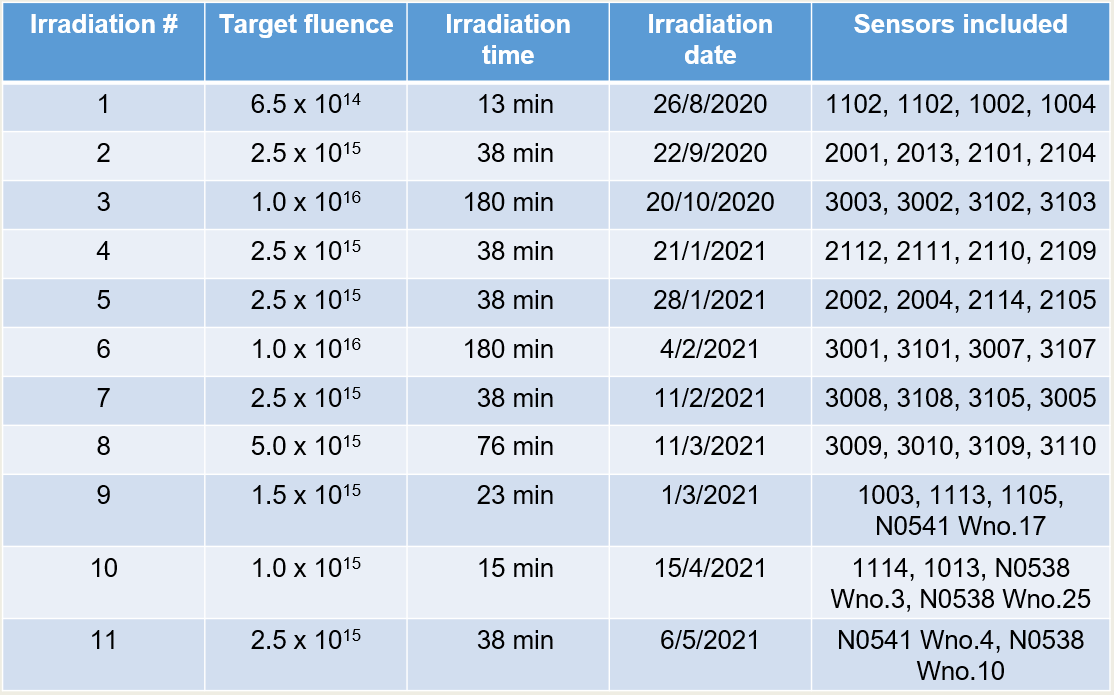
\includegraphics[width=0.90\textwidth]{figures/Completed_Irradiation_Schedule_at_RINSC}
    \caption{Completed irradiation schedule for all sensors irradiated in this campaign.}
    \label{fig:Irradiation_Schedule}
  \end{center}
\end{figure}

\begin{figure}[!hbt]
  \begin{center}
    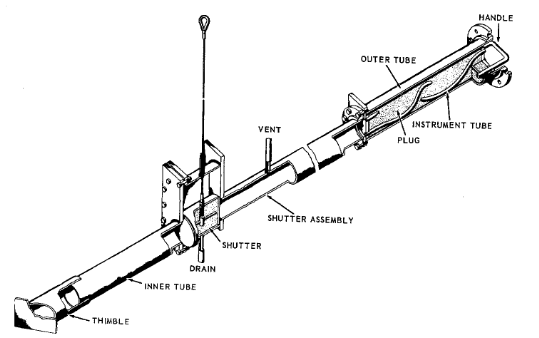
\includegraphics[width=0.80\textwidth]{figures/Beamport_Schematic}
    \caption{Schematic of one of the beamport sample delivery systems at the RINSC Facility.}
    \label{fig:Beamport_Schematic}
  \end{center}
\end{figure}

\begin{figure}[!hbt]
  \begin{center}
    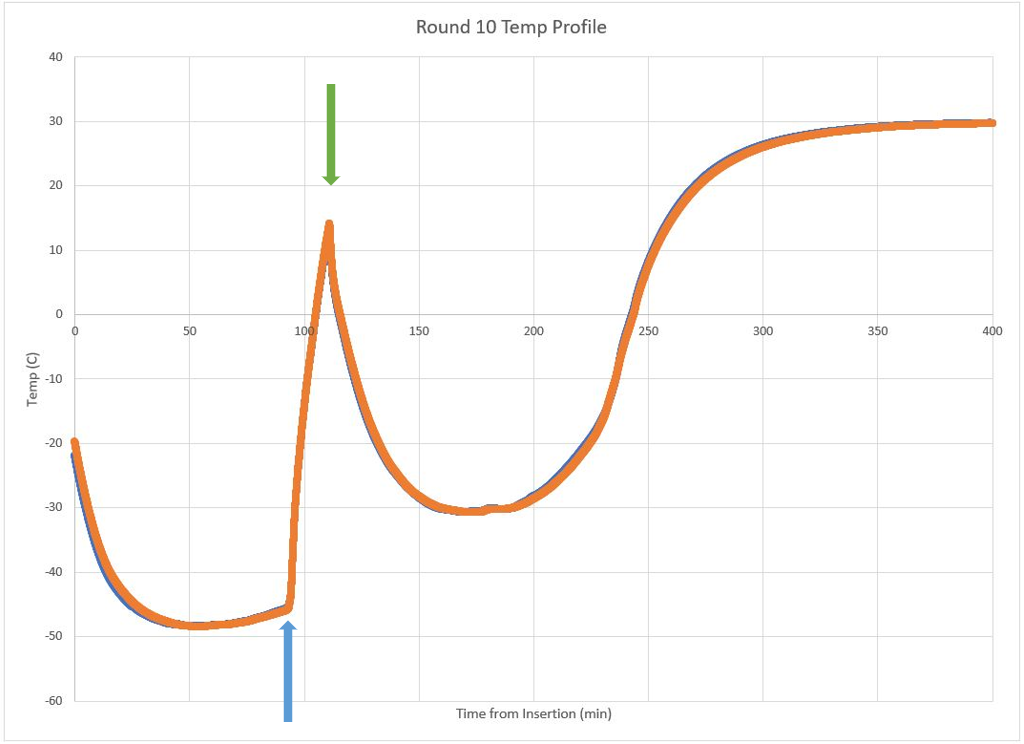
\includegraphics[width=0.80\textwidth]{figures/Round_10_Temperature_Profile}
    \caption{Temperature profile for sensor irradiation round 10. The blue arrow indicates the time at when the reactor was turned on, and the green arrow indicates at what time the reactor was shut off.}
    \label{fig:Round_10_Temperature_Profile}
  \end{center}
\end{figure}

\begin{itemize}
    \item \ref{fig:RINSC_Facility} - image(s) of reactor core, beamport (see .~\ref{fig:RINSC_Facility})
    %what other details are useful here?
    %Is it better to omit the sample irradiation options that are not being used?
    \item \ref{fig:Pucks_Arrayed} - puck design/layout, real pucks (see .~\ref{fig:Pucks_Arrayed})
    %\item Fig 3 - puck layout, packing (see .~\ref{fig:Puck_Packing}), how much detail about packing materials? (see .~\ref{fig:Cylinder_Details})
    %\item Fig 4 - other hardware, cylinder, temp monitoring setup (see .~\ref{fig:Temperature_Monitoring_Setup})
    %Keithley 2400 for temperature readout (along with 20-channel input board), RTDs instrumented with 20' of radiation-resistant wire (McMaster), laptop with GPIB connection to keithely, and custom LabVIEW code for readout.
    %\item Fig 5 - schemaitc of experimental setup? Is this needed?
    %\item describe sample removal/storage after irradiation - need for full day for activity levels to decay to the point that reactor staff can transfer cylinder from beamport to freezer. Chest freezer has been installed a few steps away from the beamport with enough storage capacity for 3 cylinders.
    %\item Fig 6 describe fluence measurement setup/procedure at Brown? IV of D0 diodes prior to irradiation, then cold (-20C) measurement of irradiated diodes with current scaled up to 20C. Also include pin diodes but they have not been found to be useful at fluences above 1e15. (see .~\ref{fig:Fluence_Measurement_Setup})
\end{itemize}

\begin{figure}[!hbt]
  \begin{center}
    %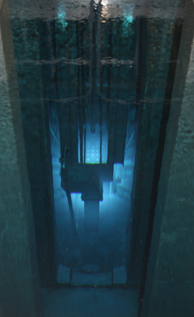
\includegraphics[width=0.25\textwidth]{figures/RINSC_Reactor_Core}
    \includegraphics[width=0.40\textwidth]{figures/Beamport_View}
    \caption{On the left is an image of the reactor core at RINSC, and on the right is a view down the beamport used for these irradiation studies.}
    \label{fig:RINSC_Facility}
  \end{center}
\end{figure}

\begin{figure}[!hbt]
  \begin{center}
    \includegraphics[width=0.70\textwidth]{figures/Hockey_Pucks_Arrayed}
    \caption{Sample containers ('hockey pucks') for sensors to be irradiated in the beamport at RINSC. The materials are wood (oak), acrylic, and PEEK.}
    \label{fig:Pucks_Arrayed}
  \end{center}
\end{figure}

\iffalse      %START OF MULTILINE COMMENT
\begin{figure}[!hbt]
  \begin{center}
    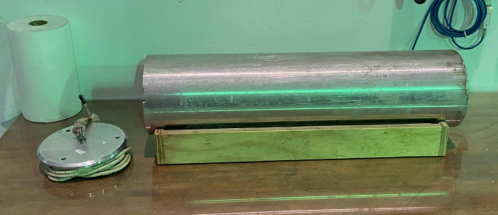
\includegraphics[width=0.60\textwidth]{figures/Cylinder_Side_View}
    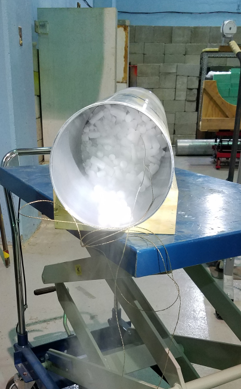
\includegraphics[width=0.30\textwidth]{figures/Cylinder_With_Dry_Ice}
    \caption{Left: aluminum cylinder used to transport hockey puck containers into the beamport. Right: cylinder containing a sample puck along with dry ice for cooling.}
    \label{fig:Cylinder_Details}
  \end{center}
\end{figure}

\begin{figure}[!hbt]
  \begin{center}
    \includegraphics[width=0.20\textwidth]{figures/Hockey_Puck_Base_Instrumented}  
    \includegraphics[width=0.25\textwidth]{figures/Hockey_Puck_Sensor_Fit}
    \includegraphics[width=0.25\textwidth]{figures/Hockey_Puck_Kapton_Layer}
    \includegraphics[width=0.20\textwidth]{figures/Hockey_Puck_Lid_Instrumented}    
    \caption{Four views of sensor container packing: the base instrumented with fluence monitoring diodes, the fit of a sensor in the hockey puck, the protection of the sensor with layers of kapton foil, and the lid of the hockey puck instrumented with monitoring devices.}
    \label{fig:Puck_Packing}
  \end{center}
\end{figure}

\begin{figure}[!hbt]
  \begin{center}
    \includegraphics[width=0.80\textwidth]{figures/Temperature_Monitoring_Setup}
    \caption{Temperature monitoring setup for use during beamport irradiations at RINSC.}
    \label{fig:Temperature_Monitoring_Setup}
  \end{center}
\end{figure}

\begin{figure}[!hbt]
  \begin{center}
    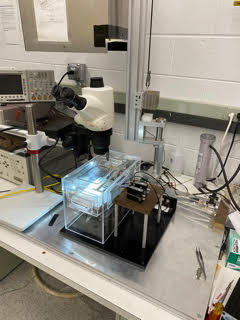
\includegraphics[width=0.35\textwidth]{figures/CVIV_Setup}
    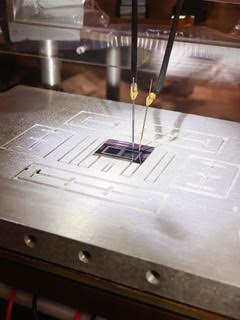
\includegraphics[width=0.35\textwidth]{figures/D0_Measurement}
    \caption{Left: measurement setup for extracting fluence values from irradiated diodes. Right: measurement of an unirradiated D0 diode.}
    \label{fig:Fluence_Measurement_Setup}
  \end{center}
\end{figure}

\fi       %END OF MULTILINE COMMENT
